% !TEX encoding = UTF-8
% !TEX TS-program = pdflatex
% !TEX root = ../tesi.tex
% !TEX spellcheck = it-IT

%**************************************************************
%\chapter{Verifica e validazione}
%\label{cap:verifica-validazione}
%**************************************************************
\chapter{Il modulo progetti}
\label{cap:modulo-progetti}
%**************************************************************

\intro{In questo capitolo verrà esposta l'implementazione e le fasi che hanno portato la creazione del modulo progetti}\\

\section{Scopo del modulo} Il modulo progetti, come quello clienti, si pone come scopo quello di creare un semplice sistema di CRUD in un database. Anche in questo caso valgono le considerazioni fatte riguardo al DB e in più è stata richiesta la possibilità di inviare mail a coloro i quali è stato assegnato il progetto e la assegnazione intelligente dei permessi di visualizzazione delle cartelle create a coloro i quali è stato assegnato un progetto.\\

Questo modulo si basa fortemente sulle tecniche e le funzioni già implementate e descritte durante l'esposizione del precedente modulo, tuttavia si è cercato di eseguire la  maggior parte del lavoro di composizione delle pagine tramite JavaScript, per testare la velocità di questa soluzione rispetto a quella adottata prima sia in termini di prestazioni che di tempi di sviluppo. Inoltre è stata inserita una integrazione con LDAP.

Il progetto punta a sfruttare il modulo di inserimento dei clienti per aggiungere nuove funzionalità.
A tale scopo, anche il modulo riguardante i clienti andrebbe aggiornato, per sfruttare tutte le funzionalità introdotte. Tuttavia il modulo clienti è completamente funzionante anche stand alone, mentre il modulo di un nuovo progetto è pensato per funzionare in abbinamento con il modulo della gestione dei clienti e necessita di esso.
\section{Presentazione generale del modulo}
Nella figura \ref{fig:cartelle-progetti} si illustra in generale quanto è stato prodotto per questo modulo. In seguito, nella descrizione di dettaglio, si indicheranno i nomi specifici dei file più importanti che sono stati creati
\begin{figure}[!ht]
\centering
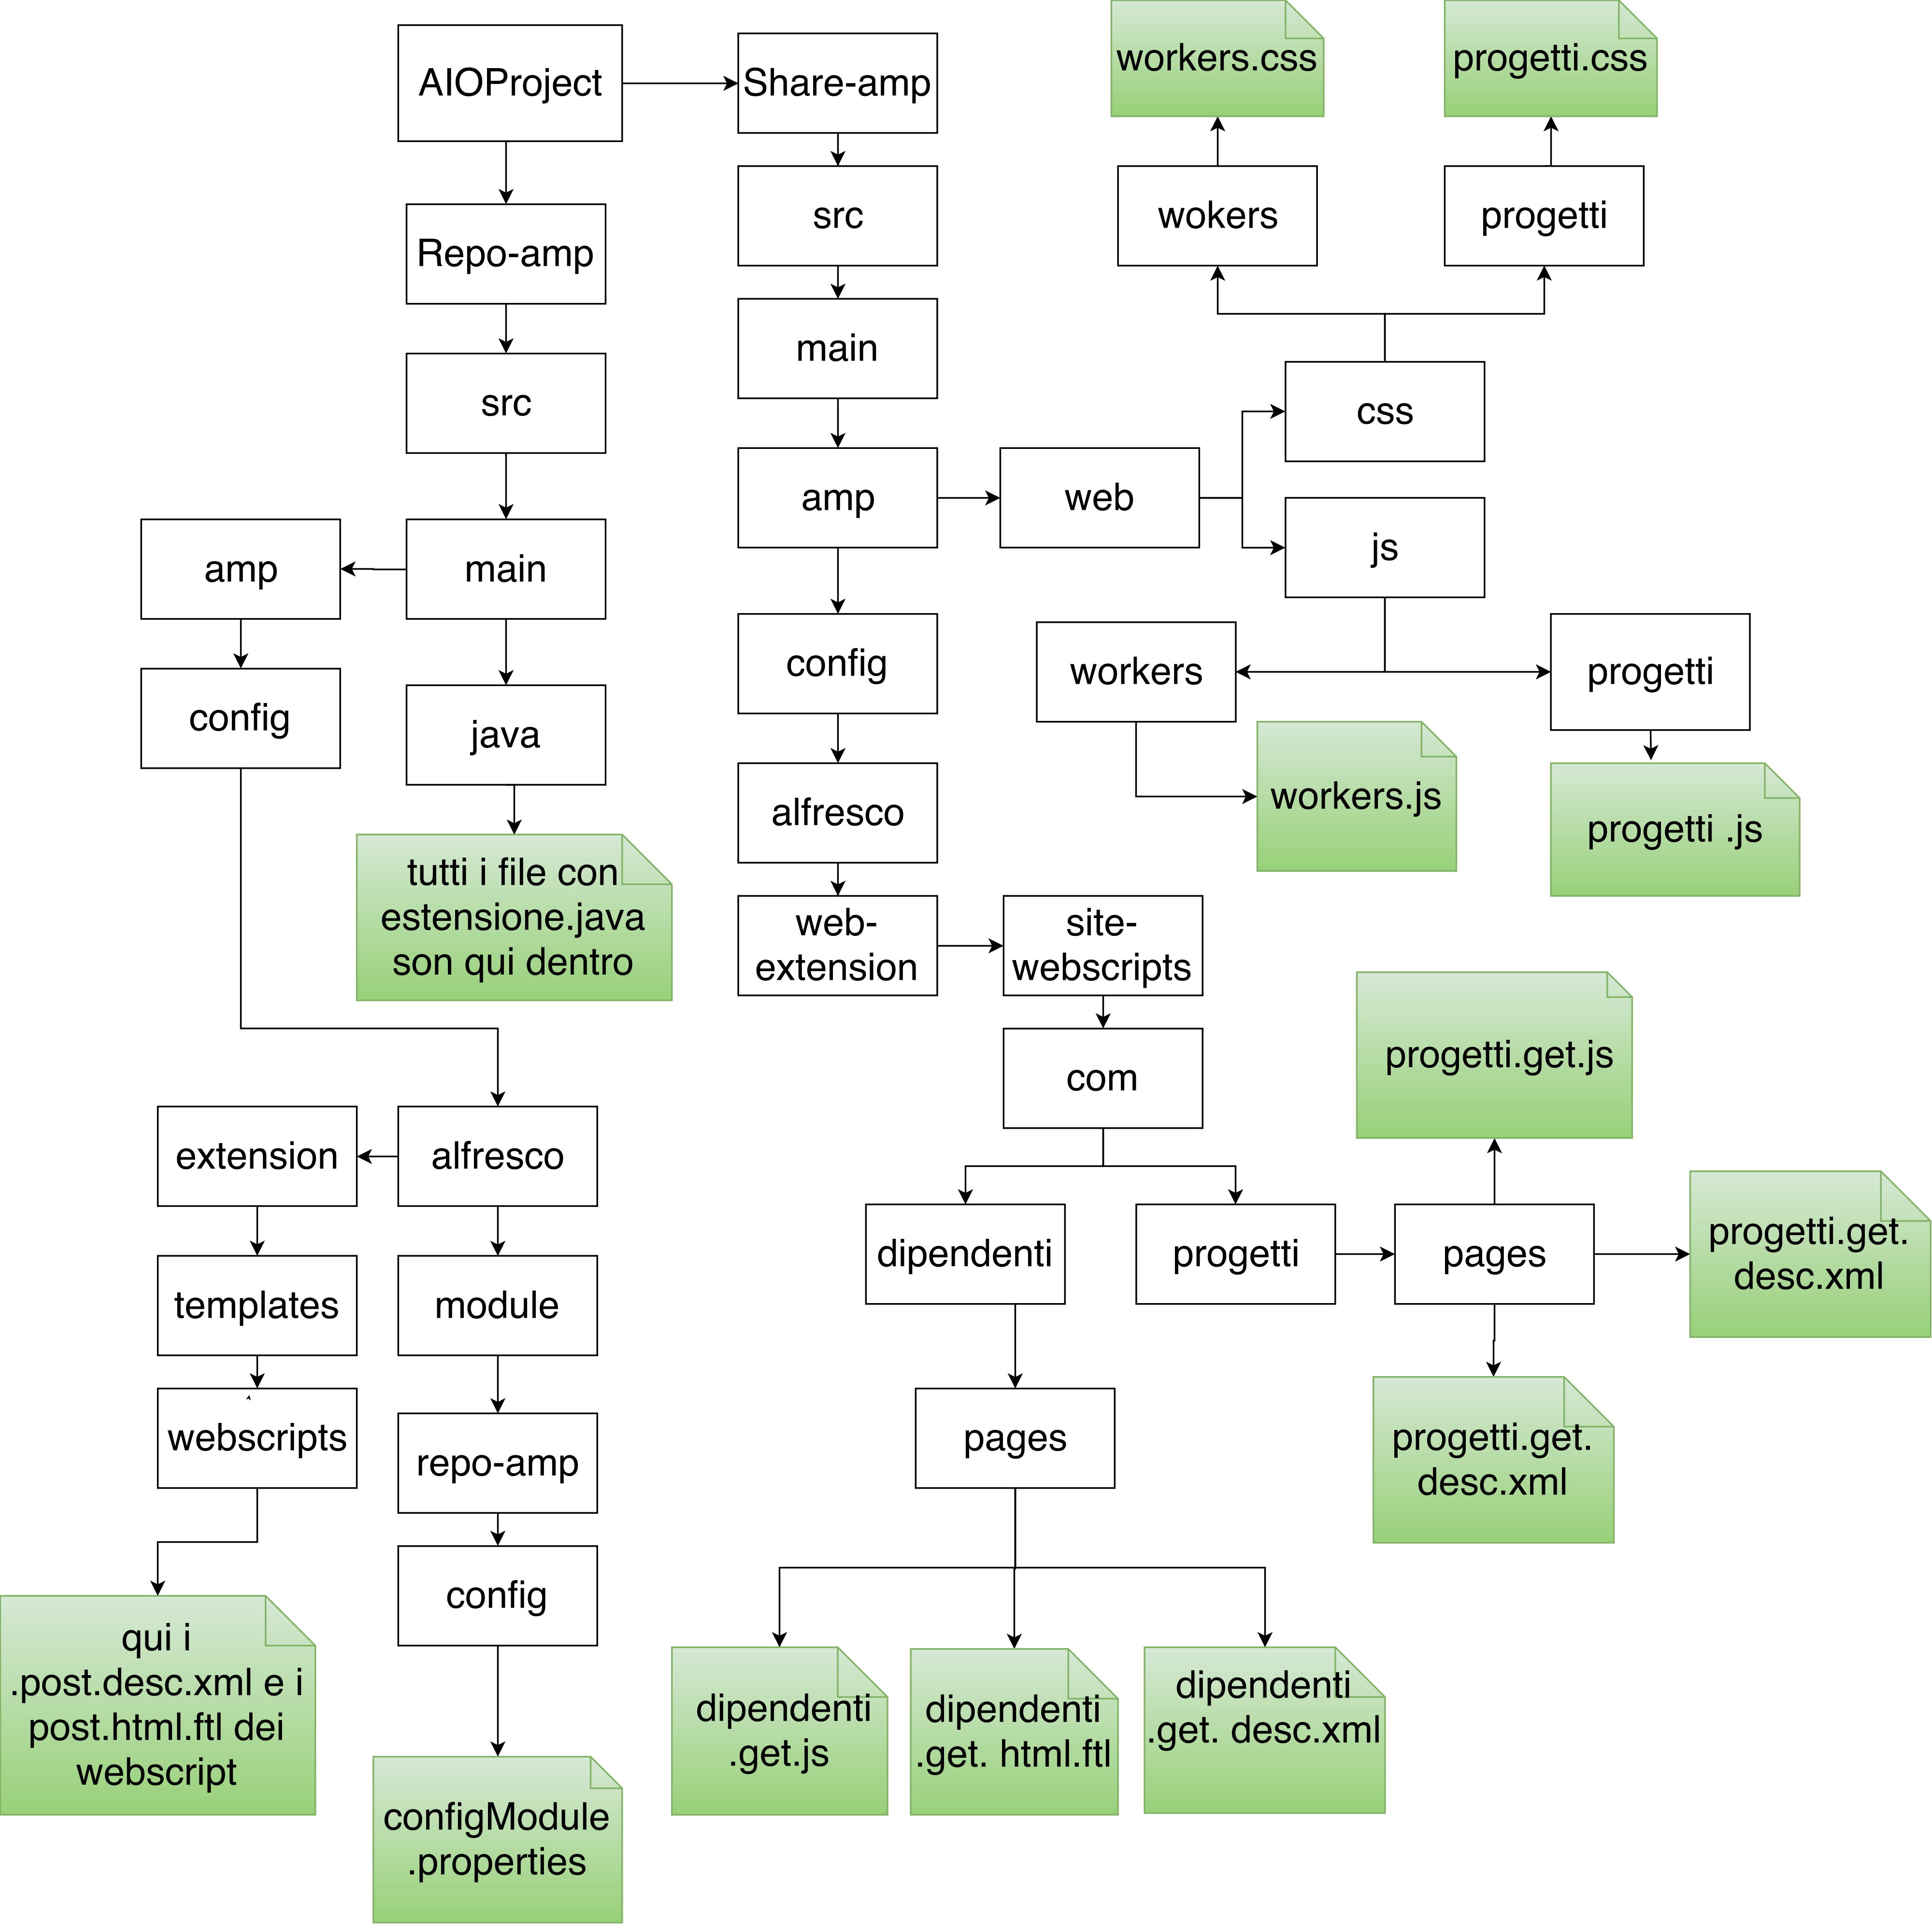
\includegraphics[width=\textwidth]{/diagrammi_cartelle/progettifolder.png}
\caption{descrizione generale di quanto creato per il modulo relativo ai progetti\label{fig:cartelle-progetti}}
\end{figure}
\section{Implementazione delle funzionalità}
\subsection{Aggiunte al DB}
Per il corretto funzionamento del modulo è stato necessario aggiungere le tabelle, il cui codice necessario per la loro generazione è riportato nei listati \ref{lst:table-progetti} e \ref{lst:table-lavoratori}
\begin{lstlisting}[language=SQL,caption=codice per la tabella progetti, label=lst:table-progetti]
CREATE TABLE progetti
(
  nome text NOT NULL,
  descr text,
  CONSTRAINT progetti_pkey PRIMARY KEY (nome)
)
\end{lstlisting}
La tabella relativa ai progetti, riportata nel listato \ref{lst:table-progetti} è una tabella che semplicemente deve contenere la lista dei progetti e la loro descrizione (si assume  che il nome di un progetto sia univoco, altrimenti basterebbe aggiungere un id in auto\_increment alla tabella). La seguente tabella è stata pensata per garantire la possibilità di aggiunta di attributi ad un progetto,  senza aggiungere complessità alla tabella di coloro che sono impiegati in un progetto.
È necessaria per poter gestire il caso di un progetto senza alcun assegnatario, ed in futuro verrà sicuramente espansa all'aggiunta di nuove funzionalità.

Più degna di nota è la tabella delle persone impegnate su un progetto, riportata nel listato \ref{lst:table-lavoratori}

\begin{lstlisting}[language=SQL,caption=codice per la tabella lavoratori, label=lst:table-lavoratori]
CREATE TABLE lavoratori
(
  mail text NOT NULL,
  project text NOT NULL,
  client serial NOT NULL,
  descr text,
  CONSTRAINT lavoratori_pkey PRIMARY KEY (mail, project, client),
  CONSTRAINT lavoratori_client_fkey FOREIGN KEY (client)
      REFERENCES clienti (id) MATCH SIMPLE
      ON UPDATE NO ACTION ON DELETE NO ACTION
)
\end{lstlisting}

Come si vede vi è qui diretto collegamento tra il progetto e il cliente che lo ha commissionato (si assume nell’assegnazione del progetto che la versione del cliente a cui viene assegnato un progetto sia quella dell’ultima modifica nota eseguita tramite il modulo clienti. Ciò è garantito del fatto di selezionare l’id maggiore, in quanto il tipo serial dell’id cliente non decresce alla cancellazione di un record; si ha quindi la certezza che ad un dato nome di un cliente, la sua ultima versione è quella con id maggiore.

\subsection{Definizione delle properties}

Il sistema fa uso delle seguenti properties, riportate nel listato \ref{lst:properties-progetti} per far capire meglio le query utilizzate.
\begin{lstlisting}[label=lst:properties-progetti,caption=properties del modulo relativo ai progetti]
#query configuration
queryselectallprojects=select project,mail,lavoratori.descr,identificativo from lavoratori join clienti on Client=ID order by project
queryselectallclients=select distinct identificativo from clienti
#do not use values in the form paramX! They may be sobstituted!
insertworker=insert into lavoratori values ('value1','value2',(select max(ID) from clienti where identificativo='value3'),'value4');
insertproject= insert into progetti values ('value2','value4')
#server configuration
serverip=localhost
serverid=alfresco
serverpassword=admin
serverport=5432
servername=testdb
servertype=postgresql
serverconnector=jdbc
ldap.authentication.java.naming.provider.url=ldap://192.168.55.73:389
#path in lucene, in the form of PATH:\"/{directory}, the "\"" character is needed 
#because without it it will be escaped by java, java alone puts the final " so 
#you must not put it when you write the query
clientinstallationpath=PATH:\"/app:company_home/st:sites/cm:er/cm:documentLibrary/cm:_x0030_2_x0020_-_x0020_Clients/cm:put_name_here/cm:_x0030_1_x0020_-_x0020_Projects
#down here you can put the names for the folder that are in the client subdirectory
folder.father.project.one=01 - Technical Documentation
folder.father.project.two=02 - Management Documentation
folder.child.one.one=01 - Analysis
folder.child.one.two=02 - Design
folder.child.one.three=03 - Communication and Marketing
folder.child.one.four=04 - Manuals and Tutorials
folder.child.one.five=05 - Reports, Records, Meeting Minutes
folder.child.two.one=01 - Project Management
folder.child.two.two=02 - Financial
folder.child.two.two.one=01 - Proposals
folder.child.two.two.two=02 - Contracts
folder.child.two.two.three=03 - Accounting
folder.child.two.two.four=04 - Invoices
\end{lstlisting}
Come si nota sono configurabili, oltre ai parametri delle varie  connessioni, anche i nomi delle cartelle e le query.

\subsection{Parte share}
La parte share si basa su una struttura simile a quella del modulo clienti. Per ragioni di tempo, non si è potuto sviluppare un modify per i progetti e la pagina di visualizzazione dei progetti è quindi un semplice dump dei dati, con però la possibilità di inviare una mail a tutti coloro che sono stati assegnati al progetto. La struttura è stata tuttavia predisposta all’aggiunta di funzionalità.

\subsubsection{Pagina di visualizzazione dei progetti}
Vista la struttura della tabella dei lavoratori, la pagina si occupa di mostrare una riorganizzazione dei dati di quella tabella per dare una migliore leggibilità.
È composta prevalentemente attraverso l’iniezione di codice HTML da parte di funzioni JavaScript che manipolano i risultati del web service che viene chiamato tramite AJAX.
La parte statica è definita nei file
\begin {itemize}
\item \texttt{dipendenti.get.desc.xml}
\item \texttt{dipendenti.get.html.ftl}
\item \texttt{dipendenti.get.js}
\end{itemize}
Il CSS è invece situato nel file \texttt{workers.css}  e il JavaScript nel file \texttt{workers.js}. In particolare sono state implementate le seguenti funzioni, oltre a quelle di \texttt{escape/encoding/decoding} di stringhe, che sistemano la codifica delle stringhe:
\begin{itemize}
\item \texttt{setup()}, chiamata al window.onload, che si occupa di fare la chiamata AJAX per ottenere il contenuto della tabella progetti, che è una stringa nella quale il contenuto delle celle è separato dai caratteri  “\#\#\#,” mentre le righe sono separate tramite i caratteri “\#\#\#;” la stringa verrà poi trasformata in codice HTML tramite la funzione
\item \texttt{parse(response)} che si occupa di ritrasformare in un array di array la stringa passata dalla funzione di setup, e di tradurre i dati contenuti in codice HTML  più leggibile e chiaro.
\item \texttt{manda\_mail(destinatari)} che si occupa di generare un piccolo form JQuery per l'inserimento del testo della mail e di fare una chiamata AJAX al servizio SendMails per mandare la mail al gruppo a cui è stato assegnato il progetto;
\end{itemize}

\subsubsection{Pagina di inserimento di un progetto}
La pagina si occupa di inserire i dati relativi al progetto, a coloro ai quali è assegnato e a creare l'insieme delle cartelle desiderate assegnando i permessi di visione alla sola cartella tecnica a coloro ai quali è stata assegnato il progetto.
La pagina che si occupa di inserire un progetto e dove è possibile assegnare utenti (viene fornita una lista di quelli presenti nell’LDAP) ad un determinato progetto è definita nella sua parte statica dai file
\begin{itemize}
\item \texttt{progetti.get.desc.xml}
\item \texttt{progetti.get.html.ftl}
\item \texttt{progetti.get.js}
\end{itemize}
Il CSS è invece situato nel file \texttt{/progetti.css} e il JavaScript nel file \texttt{progetti.js}.
Il JavaScript utilizza le variabili globali  \texttt{buttons\_unassigned},\texttt{buttons\_assigned}, e  \texttt{assigned}
 per tenere traccia  di quali bottoni sono stati premuti e quindi anche di coloro che sono stati assegnati al progetto. Implementa,  oltre alle funzioni base di manipolazione delle stringhe, anche le seguenti funzioni:
\begin{itemize}
\item \texttt{sendRequest()}, che fa il submit del form al webscript project\_creator che si occupa di eseguire il lato backend dell’inserimento.
\item \texttt{setup()}, che si occupa di fare le richieste necessarie  ad ottenere le informazione necessarie quali la lista dei clienti e la lista degli utenti registrati nell’LDAP.
\item \texttt{process\_response(res)}, che si occupa di processare la lista degli utenti LDAP fornita dalla parte repo, nello specifico di trasformarla in button HTML e di settarne l’action onclick.
\item \texttt{refresh()}, che banalmente fa il refresh dei pulsanti mostrati nell’area degli utenti disponibili e in quella degli assegnati.
\item \texttt{assign(mail)}, che assegna un utente alla lista degli utenti a cui è stato assegnato il progetto, si occupa di ricreare il codice HTML dei bottoni e di invocare la funzione \texttt{refresh()}. Implementa anche un sistema per controllare che l’utente che si tenta di assegnare non sia già stato assegnato, poichè testando l’applicativo è capitato di notare che era possibile riuscire ad essere abbastanza rapidi da premere il pulsante di un utente due volte prima che la funzione \texttt{refresh()} lo togliesse.
\item \texttt{unassign(mail)}, che si occupa di togliere un utente dalla lista di coloro ai quali è stato assegnato un progetto e di rigenerare il codice HTML dei pulsanti e di rigenerarli invocando la funzione \texttt{refresh()}
\item \texttt{ControllerTD(),ControllerMD(), ControllerF()}, che banalmente si occupano del check e uncheck e disabilitazione dei figli al cambiamento di uno dei padri nelle checkbox.
\item \texttt{aggiungi()}, che si occupa di gestire il popup per il pulsante di aggiunta di un nuovo utente assegnatario del progetto, invocando poi la funzione \texttt{assign(mail)} per generarne il codice HTML corrispondente al relativo pulsante
\end{itemize}

\subsection{Parte Repo}
In questo modulo, rispetto a quello precedentemente descritto, si è cercato di ridurre il carico nella parte repo per spostare le operazioni relative alla generazione del codice HTML necessarie per generare il codice delle tabelle nel JavaScript.\\
Tuttavia è stata necessaria l’implementazione di cinque classi Java, necessarie a interfacciarsi con i vari componenti del backend, che verranno elencate a seguito (verranno omesse le pagine e i file di configurazione dei webscript, in quanto l'implementazione, a parte il nome, è speculare a quanto già presentato nel capitolo precedente).\\
\emph{È importante ricordarsi, se si utilizza la response per ritornare codice HTML o stringhe qualsiasi, di includere il codice riportato al listato \ref{lst:fix} per settare la response correttamente}.
\begin{lstlisting}[language=Java, caption=set dell'encoding,label=lst:fix]
res.setContentType("text/html; charset=UTF-8");
res.setContentEncoding("UTF-8");
\end{lstlisting}
 Altrimenti la codifica dei caratteri non riesce in maniera corretta.
\subsubsection{Clienti.java}
Questa pagina è chiamata senza parametri tramite richiesta POST al webscript “clienti” dalla funzione “setup()” della pagina “progetti”, e si occupa di ritornare il codice HTML necessario a generare un select con i clienti, recuperati dal database, tra le varie option.
Si compone delle seguenti funzioni:
\begin{itemize}
\item \texttt{getValue(String value)}, che recupera una property con una data value
\item \texttt{inizialize\_values ()}, che inizializza le variabili utilizzate, recuperandole dalle properties.
\item \texttt{public void execute(WebScriptRequest req, WebScriptResponse res)} metodo obbligatorio che si può intendere come il metodo che viene invocato alla chiamata Ajax del webscript e che contiene le istruzioni per gestirla.
\item \texttt{execute(Connection con, String query, WebScriptResponse res)}, metodo che esegue la query.
\item \texttt{writedata(ResultSet rs, String result, Connection con)}, metodo che si occupa di ritornare il codice html necessario per generare il select e le option iterando il result set risultato dell’interrogazione del database.
\end{itemize}
\subsubsection{GetUsers.java}
Questa pagina è chiamata senza parametri tramite richiesta POST al webscript “GetUsers” dalla funzione “setup()” della pagina “progetti”, e si occupa di interrogare l’LDAP al fine di ottenere una lista di tutti gli utenti che sono registrati nell’LDAP. La lista è ritornata tramite una stringa con tutti i record separati con una serie di caratteri “sentinella” che fanno da separatori e che poi il Javascript si occupa di rimuovere e di riorganizzare. Esso è composto dalle seguenti funzioni:
\begin{itemize}
\item \texttt{public static DirContext ldapContext()}, che fa da costruttore senza parametri di un ldap context. Viene seguito da
\item \texttt{public static DirContext ldapContext (Hashtable <String,String>env)} che invece è il suo costruttore con parametri.
\item \texttt{public static String getUsers()}, che è il metodo principale della classe e che si occupa di creare la richiesta degli utenti all’LDAP e di iterare la risposta ottenuta al fine di formare una stringa che rispetti le condizioni già citate.
\item \texttt{public static String getcontextFactory()} e \texttt{public static DirContext getLdapcontext()} che  semplicemente ritornano il valore degli omonimi  parametri.
\item \texttt{public void execute(WebScriptRequest req, WebScriptResponse res)}, metodo obbligatorio che si può intendere come il metodo che viene invocato alla chiamata AJAX del webscript e che contiene le istruzioni per gestirla.
\end{itemize}
\subsubsection{GetWorkers.java}
Questa pagina è chiamata senza parametri tramite richiesta POST al webscript “GetWorkers” dalla funzione “setup()” della pagina “dipendenti”. Essa si occupa di ritornare il risultato dell’interrogazione della tabella lavoratori, con il valore delle varie celle separati da un opportuno separatore e le righe separate da un diverso separatore. Ciò permette in seguito al codice JavaScript di ricomporla in un array di array di stringhe  che è possibile iterare.
Esso si compone delle seguenti funzioni:
\begin{itemize}
\item \texttt{getValue(String value)}, che recupera una property con una data value
\item \texttt{inizialize\_values ()}, che inizializza le variabili utilizzate, recuperandole dalle properties.
\item \texttt{public void execute(WebScriptRequest req, WebScriptResponse res)} metodo obbligatorio che si può intendere come il metodo che viene invocato alla chiamata Ajax del webscript e che contiene le istruzioni per gestirla.
\item \texttt{execute(Connection con, String query, WebScriptResponse res)}, metodo che esegue la query.
\item \texttt{writedata(ResultSet rs, String result, Connection con)}, metodo che si occupa di formare la stringa di risposta che corrisponde ai criteri descritti prima.
\end{itemize}
\subsubsection{Project\_creator.java}
Questa pagina è chiamata con svariati parametri tramite richiesta POST al webscript “project\_creator” dalla funzione “sendRequest()” della pagina “progetti”. È la classe più corposa implementata in tutto il progetto. In quanto si occupa di gestire l’inserimento di un nuovo progetto nel DB e di creare le cartelle corrispondenti, assegnando nel mentre i permessi di accesso e modifica alla sola cartella di documentazione tecnica (e suoi figli) a coloro ai quali è stato assegnato il progetto, in addizione ai gruppi ai quali i permessi vengono invece dati di default.
Essa si compone delle seguenti funzioni:
\begin{itemize}
\item \texttt{private void inizialize\_values()} che inizializza i valori dei vari parametri ottenuti dalle properties.
\item \texttt{public static final String getValue(String value)} che ritorna il valore della property passata come argomento alla funzione.
\item \texttt{public void give\_permissions(String[]users, String permission,NodeRef nodeRef, PermissionService permissionService)} che è usata per dare i permessi all’array di stringhe contenente la lista degli utenti a cui è stato assegnato il progetto.\\
\emph{Dato che è possibile inserire utenti non LDAP e non di Alfresco, può succedere che l’utente a cui si danno i permessi non sia registrato da nessuna parte. Ciò non provoca problemi nel sistema in quanto Alfresco lo rappresenta nella lista dei permessi con uno spazio bianco fino al momento in cui non viene definito un utente con quello username. In quel momento comparirà il nome. Ciò è stato verificato provandolo effettivamente nell’Alfresco di test. Quindi il seguente caso è tollerato, anche se non è consigliabile ricorrere a questa pratica.}
\item \texttt{public void execute(WebScriptRequest req, WebScriptResponse res)}, che viene invocato alla chiamata AJAX e si occupa di invocare e gestire le varie operazioni compiute.
\item \texttt{private void execute(Connection con, String query)}, che esegue l’inserimento del record nelle tabelle relative agli impiegati e ai progetti.
\item \texttt{private void create\_folder\_tree(String ID, String descr, String[] workers)}, che crea iterativamente l’albero delle cartelle da istanziare assegnando i permessi di default e invocando \texttt{give\_permissions} alla creazione della cartella relativa alla documentazione tecnica.
\end{itemize}
\subsubsection{SendMails.java} che si occupa di mandare un messaggio a tutte le mail di una lista, entrambe date in input alla chiamata del servizio. Questa funzione usa le \gls{API} di Alfresco, nello specifico il mailAction, che viene istanziato con il codice visibile al listato \ref{lst:mail}
\begin{lstlisting}[language=Java,caption=set dell'actionservice per le mail,label=lst:mail]
 ActionService actionService = serviceRegistry.getActionService();
 Action mailAction = actionService.createAction(MailActionExecuter.NAME);
\end{lstlisting}
Dal servizio si possono configurare numerosi parametri quali il mittente, il CC, il CCN e praticamente tutti i parametri di una normale mail.
La classe è composta solo dalla funzione \texttt{public void execute(WebScriptRequest req, WebScriptResponse res)}, che è quella chiamata automaticamente quando si richiede il servizio e che si occupa di gestire l'aggiunta dei vari destinatari e dei parametri della mail, oltre ovviamente al suo invio.
\section{Aspetto estetico}
Dato che il sistema non è stato ancora dotato delle funzionalità di update e delete, non si è ritenuto di procedere ad allinearlo con il tema Coral Tree per il momento, quindi non sono stati prodotti mockup. È stato chiesto però di rendere gradevole la presentazione
\subsection{Risultati raggiunti}
Nelle figure \ref{fig:progetti-sopra} e \ref{fig:progetti-sotto} si può vedere l'aspetto della pagina di inserimento di un nuovo progetto, mentre nella figura \ref{fig:workers} vi è la pagina dedicata alla visualizzazione dei progetti. L'aggiunta del testo per la mail avviene tramite un pop-up JQuery.
\begin{figure}[!ht]
\centering
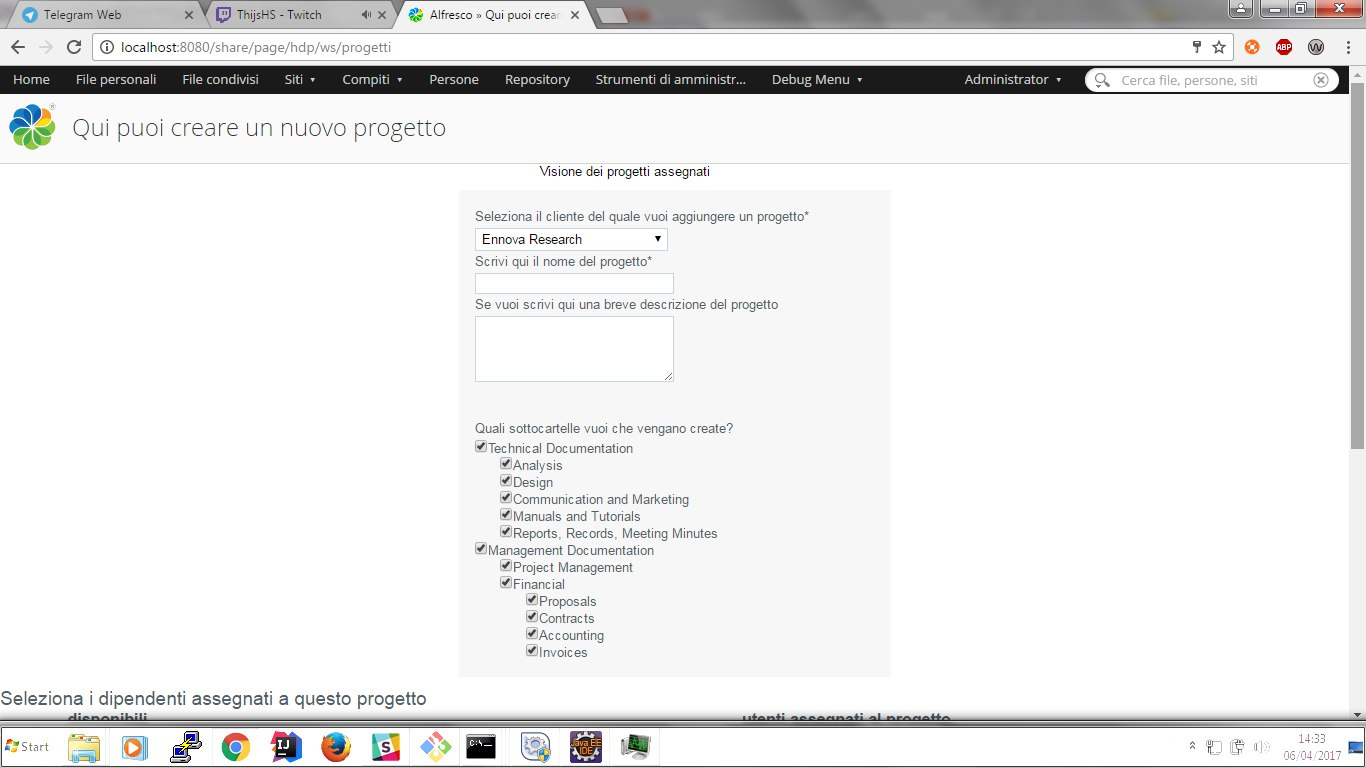
\includegraphics[width=\textwidth]{nuove_immagini/progetti-sopra}
\caption{pagina di inserimento di un nuovo progetto, inserimento dei dati\label{fig:progetti-sopra}}
\end{figure}
\begin{figure}[!ht]
\centering
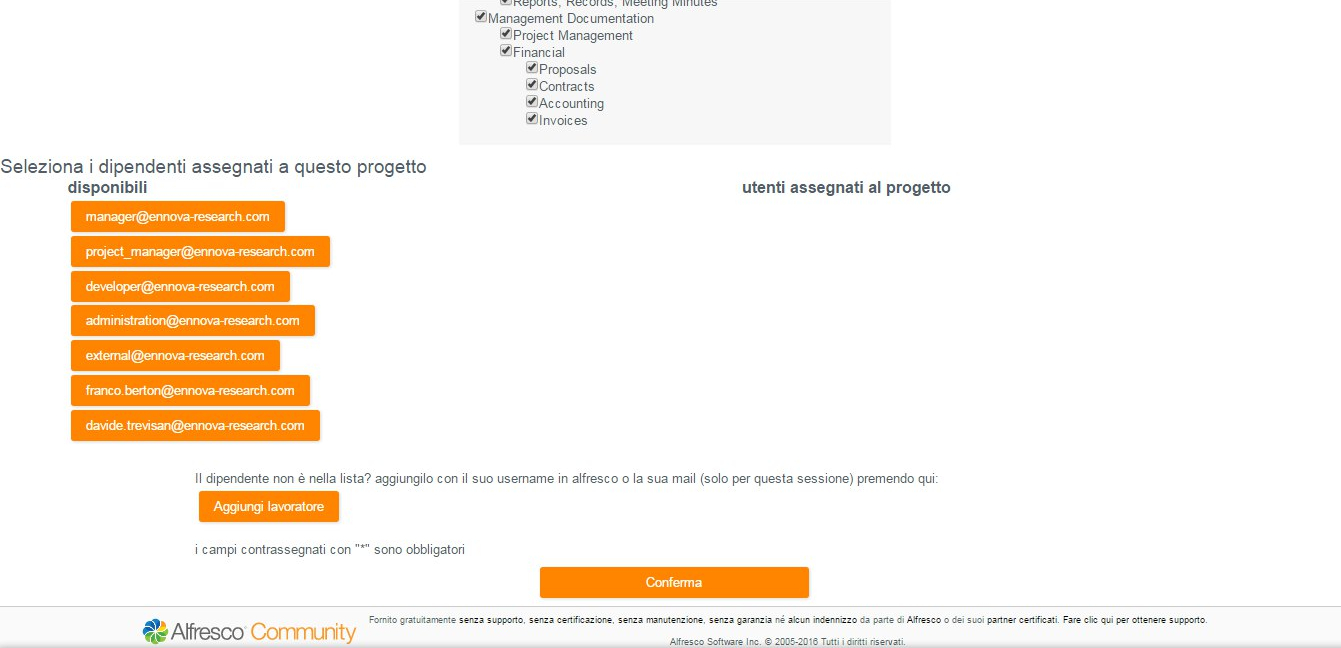
\includegraphics[width=\textwidth]{nuove_immagini/progetti-sotto}
\caption{pagina di inserimento di un nuovo progetto, assegnazione dei lavoratori \label{fig:progetti-sotto}}
\end{figure}
\begin{figure}[!ht]
\centering
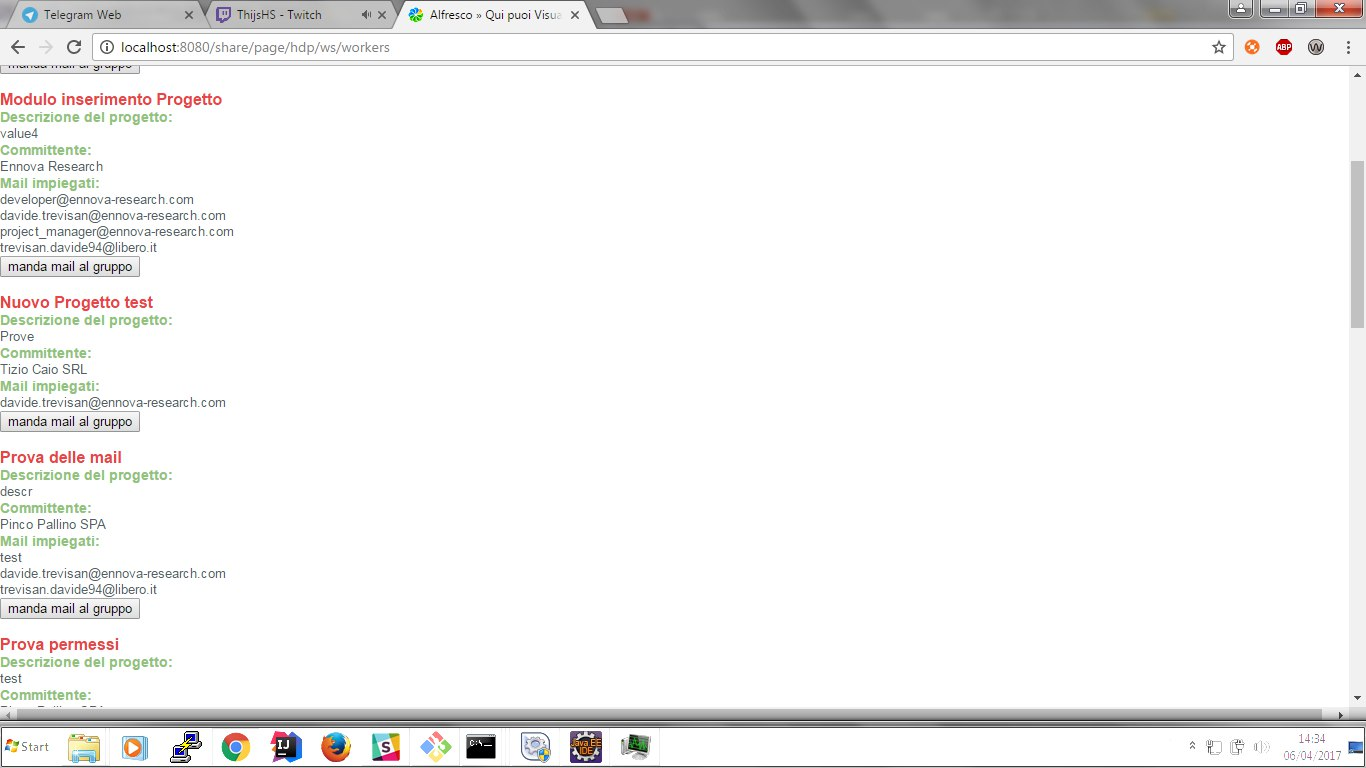
\includegraphics[width=\textwidth]{nuove_immagini/workers}
\caption{pagina di visualizzazione dei progetti \label{fig:workers}}
\end{figure}